\documentclass[a4paper]{article}

% Abbildung 11: http://www.wolframalpha.com/input/?i=x^2-5x%2B6%3E0

\usepackage[german]{babel}
\usepackage[utf8]{inputenc}
\usepackage{amsmath}
\usepackage{amssymb}
\usepackage{esvect} % vectors - vv{AB}
\usepackage{graphicx}
\usepackage{float} % fixed position for pictures - [H]
\usepackage{verbatim} % multi line comments - \begin{comment} \end{comment}

\title{Kursnotizen Mathematik 1}
\author{Josef Steppan}
\date{\today}

\begin{document}
\maketitle

\begin{abstract}
Dieses Dokument enthält Notizen aus dem Kurs Mathematik 1 des Studienbefähigungslehrgangs 2014/15 der FH Joanneum Kapfenberg.
\end{abstract}

%\setcounter{tocdepth}{1} % generate shorter table of contents
%\tableofcontents 

\section{Grundlegende Regeln der Algebra}
\subsection{Kommutativgesetz}
Das Kommutativgesetz gilt wenn die Argumente einer Operation vertauscht werden können ohne dass sich am Ergebnis etwas ändert. Mathematische Operationen die dem Kommutativgesetz unterliegen nennt man kommutativ.
\subsection{Assoziativgesetz}
Eine Verknüpfung ist assoziativ, wenn die Reihenfolge der Ausführung keine Rolle spielt.
\subsection{Distributivgesetz}
Umwandlung einer Summe in ein Produkt, auch bezeichnet als Ausklammern oder Herausheben. Das Auflösen von Klammern durch Anwenden des Distributivgesetzes wird als Ausmultiplizieren bezeichnet.
\begin{table}[b]
\centering
\begin{tabular}{l c r}
& Addition & Multiplikation \\ \hline
Kommutativgesetz & $x+y = y+x$ & $xy = yx$ \\\\
Assoziativgesetz & $(x+y)+z = x+(y+z)$ & $(xy)z = x(yz)$ \\
& $x+(y+z) = (x+y)+z$ & $x(yz) = (xy)z$ \\\\
Invers & $x+(-x) = 0$ & $x \cdot \frac{1}{x} = 1$ \\
& $-x+x = 0$ & $\frac{1}{x} \cdot x = 1$ \\
& & {\small Für $x \neq 0$} \\
\hline
& Distributivgesetz \\
& $x(y+z) = xy + xz$ und $(x+y)z = xz + yz$ \\
& Multiplikation mit Null \\
& $x \cdot 0 = 0$ und $0 \cdot x = 0$ \\
\hline
\end{tabular}
\caption{\label{tab:Algebra}Eigenschaften reeller Zahlen}
\end{table}

\section{Bruchrechnung}
\subsection{Mögliche Schreibweisen}
\[\frac{a}{b} = a\frac{1}{b}, \quad \frac{ac}{bc} = \frac{a}{b}, \quad \frac{a \div c}{b \div c} =\frac{\frac{a}{c}}{\frac{b}{c}} = \frac{a}{b} \quad (b,c \neq 0) \]
\[\frac{b}{1} = b\]
\subsection{Negative Werte}
\[\frac{-a}{b} = \frac{a}{-b} = -\frac{a}{b}, \quad \frac{-a}{-b} = \frac{a}{b} \quad (b \neq 0) \]
\subsection{Addition, Subtraktion}
\[\frac{a}{c} + \frac{b}{c} = \frac{a+b}{c}, \quad \frac{a}{c} + \frac{b}{d} = \frac{ad+bc}{cd} \quad (c,d \neq 0)  \] 
\[\frac{a}{c} - \frac{b}{c} = \frac{a-b}{c}, \quad \frac{a}{c} - \frac{b}{d} = \frac{ad-bc}{cd} \quad (c,d \neq 0) \]
\subsection{Multiplikation}
\[\frac{a}{b} \cdot \frac{c}{d} = \frac{ac}{bd} \quad (b,d \neq 0) \]
\subsection{Division}
Division durch Multiplikation mit dem Kehrwert, $\frac{a}{0}$ ist nicht definiert!
\[\frac{a}{c} \div b = \frac{\frac{a}{c}}{b} = \frac{a}{c} \cdot \frac{1}{b} \quad (b,c \neq 0) \] 
\[\frac{a}{b} \div \frac{c}{d} = \frac{\frac{a}{b}}{\frac{c}{d}} = \frac{a}{b} \cdot \frac{d}{c} \quad (b,c,d \neq 0) \]
Beweis: \[\frac{\frac{a}{b}}{\frac{c}{d}} = \frac{\frac{a}{b} \cdot \frac{d}{c}}{\frac{c}{d} \cdot \frac{d}{c}} = \frac{\frac{a}{b} \cdot \frac{d}{c}}{1} = \frac{a}{b} \cdot \frac{d}{c} \]

\section{Beispiele elementarer Regeln}
a) \[ 5(ab) = (5a)b \quad \text{durch Assoziativität} \]
b) \[ 4+r = r+4 \quad \text{durch Kommutativität} \]
c) \[ 3u + 7u = (3+7)u \quad \text{durch Distribution} \]
d) \[ (m+n) \cdot 0 = 0 \quad \text{durch Multiplikation mit Null} \]
e) \[ (-x)(-y)(-3) = -3xy \quad \text{durch Assoziativität} \]
f) \[ 2 \cdot x \cdot 3 + x = 6x + x = 7x \quad \text{durch Assoziativität, Multiplikation, Addition} \]
g) \[ \frac{\frac{2}{3}}{\frac{4}{5}} = \frac{2}{3} \cdot \frac{5}{4} = \frac{10}{12} = \frac{5}{6} \quad \text{durch Division} \]
h) \[ \frac{x+y}{x-y}-\frac{x}{y-x} = \frac{x+y}{x-y}-\frac{x}{-(x-y)} = \frac{x+y}{x-y}+\frac{x}{x-y} = \frac{2x+y}{x-y} \quad \text{durch Distribution, Addition} \]

\section{Klammerregeln}
Die Klammerregeln beschreiben in der Arithmetik und der elementaren Algebra Vorschriften zum Auflösen von Klammern in reinen Summen und Differenzen, also Ausdrücken, in denen nur plus und minus vorkommen. \\
\[a(b+c) = ab+ac\]
\[a(b-c) = ab-ac\]
\[(a+b)(a+b) = a^{2} + 2ab + b^{2}\]
\[(a-b)(a-b) = a^{2} - 2ab + b^{2}\]

\subsection{Differenz zweier Quadrate}
Eine Differenz zweier Quadrate $a^{2} - b^{2}$ kann man auch als Faktoren $(a-b)(a+b)$ schreiben. $(a+b)(a-b) = (a-b)(a+b)$ durch Kommutativität.
\[a^{2} - b^{2} = (a-b)(a+b)\]
\subsection{Beispiele für Anwendung der Klammerregeln}
a) \[(x+y)(x+y)=x^{2}+2xy+y^{2}\]
b) \[(2x+3y)(2x+3y)=(2x)^{2}+2(2x \cdot 3y) + (3y)^{2} = 4x^{2}+12xy+9y^{2} \]
c) \[(2x-y)(2x+y)=(2x)^{2}-(y)^{2} = 4x^{2}-y^{2} \]
d) \[\frac{x-y}{x^{2}-y^{2}} = \frac{(x-y)}{(x+y)(x-y)} = \frac{1}{x+y}\]
e) \[\frac{mn^{2} +m^{2}n^{3}}{mn} = \frac{mn(n+mn^{2})}{mn} = n+mn^{2}\]
f) \[\frac{2x(x-y)}{x^{3}-xy^{2}} = \frac{2x^{2}-2xy}{x(x^{2}-y^{2})} = \frac{x(2x-2y)}{x(x^{2}-y^{2})} = \frac{2x-2y}{x^{2}-y^{2}} = \frac{2(x-y)}{(x-y)(x+y)} = \frac{2}{x+y}\]
g) \[\frac{x^{3}}{2} + \frac{2x^{2}+x^{3}}{4x} = \frac{x^{2}x}{2} + \frac{x^{2}(2+x)}{2 \cdot 2x} = \frac{x^{2}}{2}(x) + \frac{x^{2}}{2} \left(\frac{2+x}{2x}\right) = \frac{x^{2}}{2} \left(x+\frac{2+x}{2x}\right) \]

\begin{table}[t]
\centering
\begin{tabular}{l} Wenn $a=b$ und $a,b,c$ reelle Zahlen\\ 
\hline
$a+c=b+c$ \\
$a-c=b-c$ \\
$ac=bc$ \\
$ \frac{a}{c} = \frac{b}{c} \quad (c \neq 0$) \\ \hline
$a=b \Leftrightarrow a^{2}=b^{2} \quad (ab \geq 0)$\\
$a=b \Leftrightarrow \sqrt{a}=\sqrt{b} \quad (ab \geq 0)$\\
$a=\sqrt{b} \Leftrightarrow a^{2} = b \quad (b \geq 0)$\\
$a \cdot b = 0 \Rightarrow a=0$ oder $b=0$ \\ 
\hline
\end{tabular}
\caption{\label{tab:Gleichungen}{Umformen von Gleichungen}}
\end{table}

\section{Lineare Gleichungen}
Eine lineare Gleichung $ax+b=0$ besitzt genau eine Lösung $x = \frac{-b}{a}$. \\ Für $a,b$ reelle Zahlen, $a\neq 0$, und $x$ unbekannt:
\begin{center} $ax+b=0$\\
$x = \frac{-b}{a}$
\end{center}

\subsection{Beispiele für die Lösung von Gleichungen}
a)
\begin{align*}
(e+f)^{2} &= (e-2f)^{2} \\
(e+f)(e+f) &= (e-2f)(e-2f) \\
e^{2}+ef+fe+f^{2} &= e^{2}-2ef-2fe+4f^{2} \\
e^{2}+2ef+f^{2} &= e^{2}-4ef+4f^{2} \\
f^{2}-4f^{2} &= -4ef - 2ef \\
-3f^{2} &= -6ef \\
e &= \frac{-3f^{2}}{-6f} = \frac{f^{2}}{3f} = \frac{f}{3} = \frac{1}{3}f
\end{align*}
b)
\begin{align*}
(x+3)(x-5)=0 \\
x=-3 \text{ oder } x=5
\end{align*}
Da mindestens einer der beiden Faktoren Null sein muss um die Gleichung zu erfüllen ist entweder (x+3) oder (x-5) Null, x daher -3 oder 5.

\section{Mengen}
Eine Menge ist eine Zusammenfassung unterscheidbarer Objekte zu einer Gesamtheit. Die Menge, die kein Element enthält, heißt leere Menge. Sie wird mit $\emptyset$ oder auch $\{\}$ bezeichnet. Die leere Menge ist Teilmenge einer jeden Menge.
\begin{figure}[H]
\centering
\includegraphics[width=0.25\textwidth]{images/teilmenge.png}
\caption{\label{fig:teilmenge}Teilmenge $A \subset B$}
\end{figure}
$A \subset B$ (Teilmenge); Eine Menge A heißt Teilmenge einer Menge B wenn jedes Element von A auch Element von B ist. Jede Menge A ist auch Teilmenge von sich selbst: $A \subseteq A $. A ist echte Teilmenge von B, wenn jedes Element aus A auch Element von B ist, aber mindestens ein Element in B existiert, das nicht in A enthalten ist. Es sind zwei Notationen für Teilmengen gebräuchlich: $A \subseteq B$ für „Teilmenge“ und $A \subset B$ für „echte Teilmenge“ 
\begin{figure}[H]
\centering
\includegraphics[width=0.25\textwidth]{images/schnittmenge.png}
\caption{\label{fig:schnittmenge}Schnittmenge $A \cap B$}
\end{figure} 
$A \cap B$ (Schnittmenge); Alle Elemente die sowohl in A als auch in B enthalten sind: $A \cap B = \{ x \mid (x \in A) \land (x \in B)\} $
\begin{figure}[H]
\centering
\includegraphics[width=0.25\textwidth]{images/vereinigungsmenge.png}
\caption{\label{fig:vereinigungsmenge}Vereinigungsmenge $A \cup B$}
\end{figure}
$A \cup B$ (Vereinigungsmenge); Alle Elemente, die in A oder in B oder in beiden enthalten sind: $A \cup B = \{ x \mid (x \in A) \lor (x \in B)\} $
\begin{figure}[H]
\centering
\includegraphics[width=0.25\textwidth]{images/differenzmenge.png}
\caption{\label{fig:differenzmenge}Differenzmenge $A \setminus B$}
\end{figure}
$A \setminus B$ (Differenzmenge); A ohne B, also alle Elemente, die in A enthalten sind, aber nicht in B: $A \setminus B = \{ x \mid (x \in A) \land (x \notin B)\} $
\begin{figure}[H]
\centering
\includegraphics[width=0.25\textwidth]{images/komplement.png}
\caption{\label{fig:komplement}$A^{\rm C}$ (Komplement von A)}
\end{figure}
$A^{\rm C} = U \setminus A$: Alle Elemente des Universums U die nicht in A liegen: $A ^{\rm C} = U \setminus A = \{ x \mid (x \in U) \land (x \notin A)\} $

\section{Aussagen}
Eine Aussage ist ein Satz, der entweder wahr (w) oder nicht wahr (f) ist. Eine Aussage die immer wahr ist, z.B. $ A \lor \neg A$, nennt man Tautologie.
\subsection{Junktoren}
In der klassischen Aussagenlogik sind die folgenden Junktoren am gebräuchlichsten:
\begin{itemize}
\item die Negation $\neg P$ entspricht einer Verneinung
\item die Implikation $P \Rightarrow Q$ entspricht der hinreichenden Bedingung: „Wenn P, dann Q“
\item das Bikonditional $\Leftrightarrow$, auch Äquivalenz genannt, ist eine zusammengesetzte Aussage, die genau dann wahr ist wenn ihre beiden Teilaussagen denselben Wahrheitswert haben, also entweder beide wahr oder beide falsch sind.
\item die Konjunktion $P \land Q$, das logische Und: „Sowohl P als auch Q“. Eine Konjunktion ist genau dann wahr wenn beide Aussagen wahr sind.
\item die Disjunktion $P \lor Q$, das einschließende Oder: „P oder Q oder beide“. Eine Disjunktion ist wahr wenn eine oder beide der Aussagen wahr sind.
\end{itemize}
\begin{tabular}{c c | c c c c c c}
A & B & $A \land B$ & $A \lor B$ & $\neg A$ & $A \Rightarrow B$ & $\neg B \Rightarrow \neg A$ & $(A \Rightarrow B) \Leftrightarrow (\neg B \Rightarrow \neg A)$ \\
\hline
w & w & w & w & f & w & w & w \\
w & f & f & w & f & f & f & w \\
f & w & f & w & w & w & w & w \\
f & f & f & f & w & w & w & w \\
\hline
\end{tabular}
\subsection{Quantoren}
Die beiden gebräuchlichsten Quantoren sind der Existenzquantor („mindestens ein“) und der Allquantor („alle“ oder „jede/r“):
\begin{itemize}
\item Der Existenzquantor $\exists$: Für (mindestens) ein/einige/manche gilt \dots
\item Der Allquantor $\forall$: Für alle/jedes gilt \dots
\end{itemize}

\section{Die Menge reeller Zahlen $\mathbb{R} = \mathbb{Q} \cup \mathbb{I}$}
Die Menge der reellen Zahlen entspricht der Menge aller Punkte der Zahlengeraden und besteht aus den rationalen Zahlen, vereinigt mit den irrationalen Zahlen: $\mathbb{R} = \mathbb{Q} \cup \mathbb{I}$ \\\\
Die natürlichen Zahlen sind enthalten in den ganzen Zahlen sind enthalten in den rationalen Zahlen sind enthalten in den reellen Zahlen: $\mathbb{N} \subset \mathbb{Z} \subset \mathbb{Q} \subset \mathbb{R}$
\subsection{Natürliche Zahlen}
Die natürlichen Zahlen sind die beim Zählen verwendeten Zahlen 1, 2, 3, 4, 5, 6, 7, 8, 9, 10 usw. Oft wird auch die 0 (Null) zu den natürlichen Zahlen gerechnet.
\[ \mathbb{N} = \{0;1;2;3;\dots\} \]
\subsection{Ganze Zahlen}
Die ganzen Zahlen sind eine Erweiterung der natürlichen Zahlen. Sie enthalten alle natürlichen Zahlen, deren Negative, und Null. \\
\[ \mathbb{Z} = \{\dots;-3;-2;-1;0;1;2;3;\dots\} \]

\subsection{Rationale Zahlen}
Eine rationale Zahl ist eine reelle Zahl die als Verhältnis zweier ganzer Zahlen dargestellt werden kann.
\[ \mathbb{Q} = \left\{\frac{p}{q} \middle| p \in \mathbb{Z}, q \in \mathbb{Z} \setminus \{0\}\right\} \]

\subsection{Irrationale Zahlen}
Eine Zahl heißt irrational, wenn sie reell, aber nicht rational ist, also nicht als Verhältnis zweier ganzer Zahlen dargestellt werden kann. Im Gegensatz zu rationalen Zahlen, die als endliche oder periodische Dezimalzahlen dargestellt werden können, sind irrationale Zahlen solche, deren Dezimaldarstellung nicht abbricht und nicht periodisch ist, z. B. $\sqrt{2}, \pi, e$.
\[ \mathbb{I} = \mathbb{R} \setminus \mathbb{Q} \]

\section{Quadratische Gleichungen}
Eine quadratische Gleichung ist eine Gleichung, die sich in der Form
\[ ax^{2}+bx+c=0 \]
mit $a \neq 0$ schreiben lässt. Hierbei sind a, b, c Koeffizienten; x ist die Unbekannte. Ist $b=0$, spricht man von einer reinquadratischen Gleichung.
\subsection{Lösung}
Eine Lösung der quadratischen Gleichung ist eine Zahl, die die Gleichung erfüllt, wenn sie für x eingesetzt wird. Jede quadratische Gleichung hat, wenn man komplexe Zahlen als Lösungen zulässt, genau zwei (gegebenenfalls zusammenfallende) Lösungen, auch Wurzeln der Gleichung genannt. Betrachtet man nur die reellen Zahlen, so hat eine quadratische Gleichung null bis zwei Lösungen.
\subsection{Anzahl der Lösungen}
Die Anzahl der Lösungen lässt sich mit Hilfe der Diskriminante D  bestimmen:
\begin{align*}
D = b^{2}-4ac
\end{align*}
\begin{figure}[h!]
\centering
\includegraphics[width=0.8\textwidth]{images/diskriminante.png}
\caption{\label{fig:diskriminante}Lage der quadratischen Parabeln und Auswirkungen auf die Zahl der Nullstellen}
\end{figure}
\begin{description}
\item[(A)] Diskriminante positiv: Die Parabel hat zwei Schnittpunkte mit der x-Achse, es gibt also zwei verschiedene reelle Nullstellen $x_{1}$ und $x_{2}$.
\item[(B)] Diskriminante Null: Die Parabel hat genau einen Berührpunkt mit der x-Achse, nämlich ihren Scheitelpunkt. Es gibt somit genau eine (doppelte) reelle Lösung. Die quadratische Gleichung lässt sich auf die Form $ax^2 + bx + c = a \cdot (x - x_1)^2 = 0$ bringen.
\item[(C)] Diskriminante negativ: Die Parabel hat keinen Schnittpunkt mit der x-Achse, es gibt keine reellen Lösungen der quadratischen Gleichung.
\end{description}

\subsection{Lösung bei fehlendem linearen Teil}
Die reinquadratische Gleichung $ax^{2}+c=0$ lässt sich durch Umformen lösen:
\begin{align*}
x_{1,2} = \pm \sqrt{-\frac{c}{a}}
\end{align*}
\subsection{Lösung bei fehlender Konstante}
Aus der Gleichung $ax^{2} + bx = 0$ ergibt sich durch Ausklammern $x(ax+b) = 0$, es muss also $x = 0$ oder $ax+b=0$ gelten. Die beiden Lösungen lauten damit
\begin{align*}
x_{1} = 0 \text{ und } x_{2}=-\frac{b}{a}
\end{align*}
\subsection{Lösung für Normalform}
Bei Vorliegen der Normalform $x^2+px+q=0$ lauten die Lösungen
\begin{align*}
x_{1,2} = - \frac{p}{2}\pm\sqrt{\left(\frac{p}2\right)^{2} - q}
\end{align*}
\subsection{Allgemeine Lösungsformel}
Die Lösungen der allgemeinen quadratischen Gleichung $ax^{2}+bx+c=0$ lauten
\begin{align*}
x_{1,2} = \frac{-b\pm\sqrt{b^2-4ac}}{2a} 
\end{align*}
\section{Satz von Vieta}
Liegt eine quadratische Gleichung in Normalform $x^2+px+q=0$ vor und hat die Lösungen $x_{1}$ und $x_{2}$, so gilt
\begin{align*}
0=x^{2}+px+q=( x -x_{1} ) \cdot ( x - x_{2} ) = x^{2} - (x_{1} + x_{2}) x + x_{1} x_{2}
\end{align*}
Durch Koeffizientenvergleich erhält man den Satz von Vieta
\begin{align*}
x_{1} + x_{2} = -p \text{ und } x_{1} \cdot x_{2} = q
\end{align*}
Besonders wenn p und q ganze Zahlen sind lassen sich so durch Ausprobieren, ob Teilerpaare von q als Summe -p ergeben die Lösungen oft rasch finden.
\subsection{Beispiel für die Anwendung des Satzes von Vieta}
Für $x^2 + 4x + 3 = 0$ gelten die Lösungen $x_{1} = -1$ und $x_{2} = -3$ \\ durch die Zerlegung $3 = (-1)(-3)$ mit $(-1) + (-3) = -4$.

\section{Umrechnung zwischen Koordinatensystemen}
\subsection{Polarkoordinaten zu kartesische Koordinaten}
Wenn man ein kartesisches Koordinatensystem mit gleichem Ursprung wie das Polarkoordinatensystem, dabei die x-Achse in der Richtung der Polarachse, und schließlich die positive y-Achse in Richtung des positiven Drehsinnes wählt, so ergibt sich für die kartesischen Koordinaten x und y eines Punktes:
\begin{align*}
x &= r\cos \varphi \\
y &= r\sin \varphi
\end{align*}
\subsection{Kartesische Koordinaten zu Polarkoordinaten}
Bestimmung des Radius r durch Anwendung des Pythagoräischen Lehrsatzes, Bestimmung des Winkels $\varphi^{\prime}$ durch Verwendung von Arcus Tangens.
\begin{align*}
r=\sqrt{x^{2}+y^{2}} \\
\varphi^{\prime}= \arctan \frac{y}{x}
\end{align*}
Die Berechnung des Winkels ist nach Lage der Koordinaten (Q1--4) unterschiedlich. Für Koordinaten in Quadrant 1 ist der Winkel $\varphi = \varphi^{\prime}$.
\begin{itemize}
\item Quadrant 1: $\varphi = \varphi^{\prime}$
\item Quadrant 2: $\varphi = 180^{\circ} - |\varphi^{\prime}|$
\item Quadrant 3: $\varphi = 180^{\circ} + |\varphi^{\prime}|$
\item Quadrant 4: $\varphi = 360^{\circ} - |\varphi^{\prime}|$
\end{itemize}

\section{Berechnungen in rechtwinkeligen Dreiecken}
Für rechtwinkelige Dreiecke gilt der Satz des Pythagoras: $c^{2}=a^{2}+b^{2}$. Die Summe der Winkel $\alpha$ und $\beta$ ergibt immer $90^{\circ}$, da $\gamma = 90^{\circ}$, und $\alpha + \beta + \gamma = 180 ^{\circ}$.
\begin{figure}[h!]
\centering
\includegraphics[width=0.6\textwidth]{images/rwdreieck.png}
\caption{\label{fig:rwdreieck}{Rechtwinkeliges Dreieck}}
\end{figure}
\begin{align*}
\sin\alpha &= \frac{a}{c} = \frac{Gegenkathete}{Hypotenuse} \\
\cos\alpha &= \frac{b}{c} = \frac{Ankathete}{Hypotenuse} \\
\tan\alpha &= \frac{a}{b} = \frac{Gegenkathete}{Ankathete} \\
\end{align*}

\section{Berechnungen in allgemeinen Dreiecken}
\begin{figure}[h!]
\centering
\includegraphics[width=0.4\textwidth]{images/dreieck.png}
\caption{\label{fig:dreieck}{Allgemeines Dreieck}}
\end{figure}
Der SSW-Fall ist nur dann eindeutig, wenn der bekannte Winkel der größeren der beiden gegebenen Seiten gegenüber liegt. Bei Angabe von Seite, Seite, Winkel (SSW) eines Dreiecks sind Null, eine, oder zwei Lösungen möglich.
\subsection{Sinussatz (SSW, SWW)}
\begin{align*}
\frac{a}{\sin\alpha}=\frac{b}{\sin\beta}=\frac{c}{\sin\gamma}
\end{align*}
\subsection{Kosinussatz (SSS, SWS)}
\begin{align*}
a^{2}=b^{2}+c^{2}-2bc\cos\alpha \\
b^{2}=a^{2}+c^{2}-2ac\cos\beta \\
c^{2}=a^{2}+b^{2}-2ab\cos\gamma
\end{align*}

\section{Lineare Funktionen}
Der Graph einer linearen Funktion ist immer eine Gerade. In kartesischen Koordinaten (x,y) erfüllen solche Geraden die Gleichung
\begin{align*}
y=kx+d
\end{align*}
Der Graph einer linearen Funktion $f$ mit $f(x)=kx+d$ ist eine Gerade mit Steigung $k$, $d$ ist der Funktionswert für $x=0$.
\subsection{Bestimmung des Funktionsterms aus zwei Punkten}
Die Steigung $k$ lässt sich berechnen zu
\begin{align*}
k = \frac{y_{2}-y_{1}}{x_{2}-x_{1}}
\end{align*}
d ergibt sich durch Auswerten von $f(0)$ oder durch Umformen zu
\begin{align*}
d=y_{1}-kx_{1} \text{ oder } d=y_{2}-kx_{2}
\end{align*}
\subsection{Schnittpunkt zweier linearer Funktionen}
Die x-Koordinate des Schnittpunktes erhält man durch Gleichsetzen beider Funktionen und Auflösen nach x, die y-Koordinate des Schnittpunktes durch das Einsetzen der erhaltenen x-Koordinate in eine der beiden Funktionen.
\begin{align*}
f(x)&=g(x)
\end{align*}
Beispiel: Schnittpunkt der Funktionen $f(x)=2x+3$ und $g(x)=3x-7$
\begin{align*}
2x+3&=3x-7 \\
x&=10
\end{align*}
Die y-Koordinate des Schnittpunktes ergibt sich aus
\begin{align*}
&y=f(10)=2(10)+3=23 \\ 
\text{ oder } &y=g(10)=3(10)-7=23
\end{align*}

\section{Lineare Gleichungssysteme in zwei Variablen}
Ein lineares Gleichungssystem mit zwei Variablen hat die Form
\[ 
\left\{
\begin{array}{l}
a_{1}x+a_{2}y=a_{0} \\
b_{1}x+b_{2}y=b_{0}
\end{array}
\right.
\]
Ein Zahlenpaar $(x \mid y)$ heisst Lösung des Gleichungssystems, wenn die reellen Zahlen x und y beide Gleichungen erfüllen.

\subsection{Lösung linearer Gleichungssysteme}
Lineare Gleichungssysteme lassen sich graphisch oder rechnerisch durch Substitution (Einsetzen), Elimination (Addition) oder Komparation (Gleichsetzen) lösen.

\subsubsection{Substitutionsmethode}
Aus einer Gleichung wird eine Unbekannte durch die andere ausgedrückt. Der erhaltene Ausdruck wird in die andere Gleichung eingesetzt.
\[
\left\{
\begin{array}{ll}
x+2y=8 & \text{\textcircled{\footnotesize{1}} } x=8-2y\\
3x+y=9 & \text{\textcircled{\footnotesize{2}}}
\end{array}
\right.
\]
Einsetzen x aus \textcircled{\footnotesize{1}} in \textcircled{\footnotesize{2}}, Auflösen nach y
\begin{align*}
3(8-2y)+y&=9 \\
24-6y+y&=9 \\
24-5y&=9 \\
5y&=15 \\
y&=3
\end{align*}
Einsetzen y in \textcircled{\footnotesize{2}}, Auflösen nach x
\begin{align*}
3x+3&=9 \\
x&=2
\end{align*}
Lösung $(2\mid 3)$

\subsubsection{Eliminationsmethode}
Man multipliziert die Gleichungen mit geeigneten Zahlen, sodass beim Addieren der beiden Gleichungen eine Unbekannte wegfällt.
\[
\left\{
\begin{array}{ll}
x+2y=8 & \text{\textcircled{\footnotesize{1}} } \cdot (-3)\\
3x+y=9 & \text{\textcircled{\footnotesize{2}}}
\end{array}
\right.
\]
Multiplikation von \textcircled{\footnotesize{1}} mit (-3)
\[
\left\{
\begin{array}{ll}
-3x-6y=-24 & \text{\textcircled{\footnotesize{3}} }\\
\hspace{13pt} 3x+y=9 & \text{\textcircled{\footnotesize{4}}}
\end{array}
\right.
\]
Addition von \textcircled{\footnotesize{3}} und \textcircled{\footnotesize{4}}, Auflösen nach y
\begin{align*}
0x-5y&=-15 \\
y&=3
\end{align*}
Einsetzen y in \textcircled{\footnotesize{2}}, Auflösen nach x
\begin{align*}
3x+3&=9 \\
x&=2
\end{align*}
Lösung $(2\mid 3)$
\subsubsection{Komparationsmethode}
Aus beiden Gleichungen wird eine Unbekannte durch die andere ausgedrückt. Anschliessend werden die erhaltenen Ausdrücke gleichgesetzt.
\[
\left\{
\begin{array}{ll}
x+2y=8 & \text{\textcircled{\footnotesize{1}} } x=8-2y\\
3x+y=9 & \text{\textcircled{\footnotesize{2}} } x=3-\frac{1}{3}y
\end{array}
\right.
\]
Gleichsetzen von x aus \textcircled{\footnotesize{1}} und x aus \textcircled{\footnotesize{2}}, Auflösen nach y
\begin{align*}
8-2y&=3-\frac{1}{3}y \\
8-3&=2y-\frac{1}{3}y \\
5&=\frac{6}{3}y-\frac{1}{3}y \\
5&=\frac{5}{3}y \\
y&=3
\end{align*}
Einsetzen y in \textcircled{\footnotesize{2}}, Auflösen nach x
\begin{align*}
3x+3&=9 \\
x&=2
\end{align*}
Lösung $(2\mid 3)$

\section{Quadratische Funktionen}
Eine quadratische Funktion hat die Form
\begin{align*}
f(x)=ax^{2}+bx+c \quad(a \neq 0)
\end{align*}
\subsection{Graph einer quadratischen Funktion}
Der Graph ist eine Parabel mit der Gleichung $y=ax^{2}+bx+c$. Die Koeffizienten a, b und c bestimmen den Wertebereich und die Form des Graphen:
\begin{itemize}
\item $a>0$: der Graph ist nach oben geöffnet
\item $a<0$: der Graph ist nach unten geöffnet
\item $|a| < 1$: der Graph ist in Richtung der y-Achse gestaucht, d. h. in der Länge zusammengedrückt, wodurch er breiter erscheint und flacher ist.
\item $|a| > 1$: der Graph ist in Richtung der y-Achse gestreckt, d. h. in die Länge gezogen, wodurch er schmaler erscheint und steiler ist. 
\end{itemize}
Eine Veränderung des Parameters c bewirkt eine Verschiebung in y-Richtung, Parameter b bewirkt eine Verschiebung sowohl in x- als auch in y-Richtung.

\subsection{Scheitelpunkt einer quadratischen Funktion}
Die Koordinaten des Scheitelpunkts S ergeben sich zu
\begin{align*}
S=\left( \frac{-b}{2a} \middle| c-\frac{b^{2}}{4a} \right)
\end{align*}
\subsection{Nullstellen einer quadratischen Funktion}
Um die Nullstellen der quadratischen Funktion zu berechnen, muss man die quadratische Gleichung gleich Null setzen ($ax^2 + bx + c = 0$) und nach x auflösen.

\section{Vektoren im zweidimensionalen Raum $\mathbb{R}^2$}
In kartesischen Koordinaten werden Vektoren durch Zahlenpaare dargestellt, die untereinander als Spaltenvektoren geschrieben werden. Zur Unterscheidung werden Punkte mit Großbuchstaben, Vektoren in Kleinbuchstaben mit einem Pfeil darüber notiert. Ortsvektoren (Ursprung am Nullpunkt des Koordinatensystems) können jedoch auch als Punkte interpretiert werden.
\[
\vec{a} = \vv{AB} = B-A
\]
\begin{figure}[H]
\centering
\includegraphics[width=0.3\textwidth]{images/vektor.png}
\caption{\label{fig:vektor}Vektor $\vec a$ mit Betrag $|\vec{a}|$ von Punkt A nach Punkt B}
\end{figure}

\subsection{Addition und Subtraktion}
Für die Addition von Vektoren gilt das Kommutativ- und Assoziativgesetz.
\[
\vec a \pm \vec b=\begin{pmatrix}a_1\\a_2 \end{pmatrix} \pm \begin{pmatrix}b_1\\b_2 \end{pmatrix}=\begin{pmatrix}a_1 \pm b_1\\a_2 \pm b_2 \end{pmatrix} 
\]
\subsection{Multiplikation mit einem Skalar}
Vektoren können mit reellen Zahlen (Skalare) multipliziert werden.
\[
r\vec a=r\begin{pmatrix}a_1\\a_2 \end{pmatrix}=\begin{pmatrix}ra_1\\ra_2 \end{pmatrix}
\]
\subsection{Multiplikation von Vektoren}
Das Produkt zweier Vektoren wird Skalarprodukt genannt. Das Ergebnis ist ein Skalar.
\[
\vec a \cdot \vec b=\begin{pmatrix}a_1\\a_2 \end{pmatrix} \cdot \begin{pmatrix}b_1\\b_2 \end{pmatrix}=a_1b_1+a_2b_2
\]
\subsection{Betrag eines Vektors}
Der Betrag bzw. die Länge eines Vektors kann durch den Satz des Pythagoras berechnet werden.
\[
|\vec a| = \sqrt{a_1^2 + a_2^2}
\]
\subsection{Orthogonalität}
Zwei Vektoren $\vec a$ und $\vec b$ heissen orthogonal (zueinander im rechten Winkel), wenn ihr Skalarprodukt Null ist.
\[
\vec a \perp \vec b \Leftrightarrow \vec a \cdot \vec b = 0
\]
\subsection{Parallelität}
Zwei von 0 verschiedene Vektoren $\vec a$ und $\vec b$ sind zueinander parallel wenn sie Vielfache voneinander sind, es also einen Skalar $r \neq 0$ gibt, so dass $\vec b = r\vec a$.
\[
\vec a \parallel \vec b \Leftrightarrow \vec b = r \vec a
\]
\subsection{Einheitsvektor}
Ein Einheitsvektor ist ein Vektor der Länge Eins. Der Einheitsvektor eines Vektors wird durch Division des Vektors durch seinen Betrag berechnet.
\[
a_0 = \frac{\vec a}{|\vec a|}
\]
\subsection{Winkelmaß zwischen zwei Vektoren}
Ist $\varphi$ das Winkelmaß der Vektoren $\vec a, \vec b \in \mathbb{R}^2$, dann gilt
\[
\cos \varphi = \frac{\vec a \cdot \vec b}{|\vec a|\cdot|\vec b|} \quad (0^{\circ} \leq \varphi \leq 180^{\circ})
\]

\section{Geraden in $\mathbb{R}^2$}
Geraden können durch ihren Funktionsterm, in Parameterdarstellung oder auch in Normalvektordarstellung beschrieben werden.

\subsection{Parameterdarstellung}
In der Parameterform wird eine Gerade in der Ebene durch einen Stützvektor $\vec p$ und einen Richtungsvektor $\vec u$ beschrieben. Eine Gerade besteht dann aus denjenigen Punkten in der Ebene, deren Ortsvektoren $\vec x$ auf $\vec p + s\vec u$ liegen.
\[
\vec x = \vec p + s\vec u \quad (s\in \mathbb{R})
\]
\begin{figure}[H]
\centering
\includegraphics[width=0.5\textwidth]{images/parameterdarstellung_gerade.png}
\caption{\label{fig:parameterdarstellung_gerade}Parameterdarstellung einer Geraden}
\end{figure}
Die Parameterdarstellung einer Geraden hat damit die Form
\[
\begin{pmatrix} x_1 \\ x_2 \end{pmatrix}=\begin{pmatrix} p_1 \\ p_2 \end{pmatrix} + s\begin{pmatrix} u_1 \\ u_2\end{pmatrix}
\]
\subsubsection{Beispiel für Schnittpunkt zweier Geraden}
\begin{align*}
g: \quad \begin{pmatrix}x\\y\end{pmatrix}&=\begin{pmatrix}1\\2\end{pmatrix}+t\cdot \begin{pmatrix}1\\1\end{pmatrix}\\
h: \quad \begin{pmatrix}x\\y\end{pmatrix}&=\begin{pmatrix}3\\4\end{pmatrix}+u\cdot \begin{pmatrix}2\\3\end{pmatrix}
\end{align*}
Gleichsetzen
\begin{align*}
\begin{pmatrix}1\\2\end{pmatrix}+\begin{pmatrix}t\\t\end{pmatrix}&=\begin{pmatrix}3\\4\end{pmatrix}+\begin{pmatrix}2u\\3u\end{pmatrix}
\end{align*}
Lösen durch Substitution
\[
\left\{
\begin{array}{ll}
1+t=3+2u & \text{\textcircled{\footnotesize{1}} } t=2+2u\\
2+t=4+3u & \text{\textcircled{\footnotesize{2}} }
\end{array}
\right.
\]
Einsetzen t aus \textcircled{\footnotesize{1}} in \textcircled{\footnotesize{2}}, Auflösen nach u
\begin{align*}
2+2+2u&=4+3u \\
u=0
\end{align*}
Einsetzen u in \textcircled{\footnotesize{1}}, Auflösen nach t
\begin{align*}
t&=3+2u-1\\
t&=2
\end{align*}
Schnittpunkt durch Einsetzen von t in g bei $\begin{pmatrix}x\\y\end{pmatrix}=\begin{pmatrix}1\\2\end{pmatrix}+\begin{pmatrix}2\\2\end{pmatrix}=\begin{pmatrix}3\\4\end{pmatrix}$


\subsection{Normalvektordarstellung}
Normalvektordarstellung der Geraden g mit Richtung $\vec g$. X und P sind Punkte auf der Geraden g, der Normalvektor $\vec n$ steht im rechten Winkel zu $\vec g$.
\[
\vec n \cdot X = \vec n \cdot P
\]

\subsubsection{Beispiel für Normalvektordarstellung}
Gegeben ist eine Gerade g mit Vektor $\vec g = \begin{pmatrix}1\\2\end{pmatrix}$ und ein Punkt $P=\begin{pmatrix}2\\3\end{pmatrix}$ auf g.\\
Der Normalvektor ist damit $\vec n = \begin{pmatrix}2\\-1\end{pmatrix}$ oder $\vec n = \begin{pmatrix}-2\\1\end{pmatrix}$, da $ \vec n \perp \vec g \Leftrightarrow \vec n \cdot \vec g=0$.\\
\begin{align*}
X \cdot \vec n&=P \cdot \vec n \\
\begin{pmatrix}x\\y\end{pmatrix}\begin{pmatrix}2\\-1\end{pmatrix}&=\begin{pmatrix}2\\3\end{pmatrix}\begin{pmatrix}2\\-1\end{pmatrix} \\
2x-y&=1 \\
y&=2x-1
\end{align*} 

\section{Logarithmen}
Wird die Eulersche Zahl e als Basis des Logarithmus verwendet so nennt man ihn den natürlichen Logarithmus. Der natürliche Logarithmus wird durch „ln“ abgekürzt. Der Logarithmus ist für 0 und negative Zahlen nicht definiert.
\[
log_a x =y \Leftrightarrow a^y=x \quad (a,x > 0, a \neq 1)
\]
\subsection{Beispiele für die Berechnung von Logarithmen}
a) 
\begin{align*}
log_{16}\frac{1}{4} = y \Leftrightarrow 16^y&=\frac{1}{4} \\
{(4^2)}^y&=4^{-1} \\
4^{2y}&=4^{-1} \\
2y&=-1 \Rightarrow y=-\frac{1}{2}
\end{align*}
b) 
\[
log_2 24 - log_2 3 = log_2 {\frac{24}{3}} =log_2 8= 3
\]
c)
\begin{align*}
2^x=7 \Leftrightarrow \log_27 &= x \\
x &= \frac{\ln7}{\ln2}
\end{align*}
d) \[\log_327=\log_3{(9\cdot3)}=\log_39+\log_33=2+1=3 \]

\begin{table}[t]
\renewcommand*{\arraystretch}{1.4}
\centering
\begin{tabular}{l l} \hline
Logarithmus eines Produkts & $\log_a (mn) = \log_a m + \log_a n$ \\
Logarithmus eines Quotienten & $\log_a \frac{m}{n}  = \log_a m - \log_a n$ \\
Logarithmus einer Potenz  & $\log_a m^p = p \log_a m$ \\
\hline
Änderung der Basis & $\log_a b = \frac{\log_c b}{\log_c a} \quad(a,c \neq 1)$ \\
Logarithmus von Eins & $\log_a 1 = 0$ \\
\end{tabular}
\caption{\label{tab:Logarithmen}{Eigenschaften von Logarithmen}}
\end{table}

\section{Wurzeln}
Die Rechenregeln für Wurzeln ergeben sich aus jenen für Potenzen. Gerade Wurzeln aus negativen Zahlen sind nicht definiert.
\[ (\sqrt[n] a)^n =a \quad (a\geq0,n\geq 1) \]
Für ungerade (3,5,7, \ldots) Zahlen 2n+1 gilt
\[ \sqrt[2n+1]{-a} = -\sqrt[2n+1]{a} \]
Für gerade (2,4,6, \ldots) Zahlen 2n gilt
\[ \sqrt[2n]{x^{2n}} = |x| \quad (x > 0) \]

\subsection{Beispiel für die Berechnung von Wurzeln}
\begin{align*}
\frac{\sqrt{\sqrt[5]{u^2v^2}}}{\sqrt[5]{v^2\sqrt{uv}}} &= \frac{{(u^2v^2)}^{\frac{1}{5}\cdot\frac{1}{2}}}{{(v^2u^{\frac{1}{2}}v^{\frac{1}{2}})}^{\frac{1}{5}}} = \frac{u^{2\cdot\frac{1}{10}}v^{2\cdot\frac{1}{10}}}{v^{2\cdot\frac{1}{5}}u^{\frac{1}{2}\cdot\frac{1}{5}}v^{\frac{1}{2}\cdot\frac{1}{5}}} = \frac{u^{\frac{1}{5}}v^{\frac{1}{5}}}{v^{\frac{2}{5}}u^{\frac{1}{10}}v^{\frac{1}{10}}} = \frac{u^{\frac{1}{5}}v^{\frac{1}{5}}}{v^{\frac{4}{10}+\frac{1}{10}}u^{\frac{1}{10}}} = \frac{u^{\frac{1}{5}}v^{\frac{1}{5}}}{v^{\frac{1}{2}}u^{\frac{1}{10}}} \\ &= u^{\frac{1}{5}-\frac{1}{10}}v^{\frac{1}{5}-\frac{1}{2}} = u^{\frac{2}{10}-\frac{1}{10}}v^{\frac{2}{10}-\frac{5}{10}} = u^{\frac{1}{10}}v^{-\frac{3}{10}}  
\end{align*}

\begin{table}[t]
\renewcommand*{\arraystretch}{1.4}
\centering
\begin{tabular}{l l l} \hline
$\sqrt[n]a \cdot \sqrt[n]b = \sqrt[n]{ab}$ & Produktregel & $\sqrt[2]2 \cdot \sqrt[2]8 = \sqrt[2]{16}$ \\
$\sqrt[m]{\sqrt[n]a} = \sqrt[mn]a$ & Wurzel einer Wurzel & $\sqrt[2]{\sqrt[3]{64}} = \sqrt[6]{64}$ \\
$\frac{\sqrt[n]a}{\sqrt[n]b} = \sqrt[n]{\frac{a}{b}}$ & Wurzel eines Quotienten & $\frac{\sqrt[3]{16}}{\sqrt[3]2} = \sqrt[3]{\frac{16}{2}}$ \\
$a^{\frac{m}{n}} = \sqrt[n]{a^m} = (\sqrt[n]a)^m$ & Rationaler Exponent& $8^{\frac{1}{3}} = \sqrt[3]8$ \\
$a^{-\frac{m}{n}} = \frac{1}{\sqrt[n]{a^m}} = \frac{1}{(\sqrt[n]a)^m} $ & Negativer rationaler Exponent & $8^{-\frac{1}{3}} = \frac{1}{\sqrt[3]8}$ \\
\hline
\end{tabular}
\caption{\label{tab:Wurzeln}{Rechenregeln für Wurzeln}}
\end{table}

\begin{table}[b]
\renewcommand*{\arraystretch}{1.4}
\centering
\begin{tabular}{l l l} \hline
$a^{n}a^{m} = a^{n+m}$  & Produktregel & $a^{2}a^{3} = a^{2+3} = a^{5}$ \\
$(a^{n})^{m} = a^{nm}$ & Potenz einer Potenz & $(a^{2})^{3} = a^{2\cdot3} = a^{6}$ \\
$(ab)^{m} = a^{m}b^{m}$ & Potenz eines Produkts & $(ab)^{2} = a^{2}b^{2}$ \\
$(\frac{a}{b})^{m} = \frac{a^{m}}{b^{m}}, b \neq 0$ & Potenz eines Quotienten & $(\frac{a}{b})^{3} = \frac{a^{3}}{b^{3}}$ \\
$\frac{a^{m}}{a^{n}} = a^{m-n} $ & Quotientenregel & $\frac{a^{5}}{a^{2}} = a^{5-2} = a^{3}$ \\
$a^{0} = 1,a \neq 0$ & Null Exponent Regel & $3^{0} = 1$ \\
$a^{-n} = \frac{1}{a^{n}}$ & Negativer Exponent & $a^{-3} = \frac{1}{a^{3}}$ \\
\hline
\end{tabular}
\caption{\label{tab:Exponenten}{Eigenschaften ganzzahliger Exponenten}}
\end{table}

\section{Exponential- und Logarithmusgleichungen}
Exponentialgleichungen lassen sich durch Logarithmieren oder Gleichsetzen der Basis lösen. Logarithmusgleichungen sind durch Exponenzieren lösbar.
\[ a^x=a^y \Rightarrow x=y \]
\[ a^x =b^y \Rightarrow x\log a =y \log b \quad(a,b >0) \]

\subsection{Beispiele für Exponential/Logarithmusgleichungen}
a) \begin{align*}
2^{3x-1}&=\frac{1}{8} & \log_2x + \log_2 6 &=4 \\
\log_2 2^{3x-1}&=\log_2 \frac{1}{8} & \log_2{(6x)} &= 4 \\
(3x-1)\log_22&=-3 & 2^4 &= 6x \\
3x-1&=-3 & 16 &= 6x \\
x&=-\frac{2}{3} & x &=\frac{8}{3}
\end{align*}
b) \begin{align*}
\log_2x^2+3\log_2x&=16 & \log_2x-2\log_2x^\frac{1}{2} = 1 \\
\log_2x^2+\log_2x^3&=16 & \log_2x-\log_2x^{\frac{1}{2}\cdot2} = 1  \\
\log_2{(x^2x^3)} &= 16 & \log_2x-\log_2x=1 \\
\log_2x^5&=16 \Leftrightarrow 2^{16} = x^5 & 0 = 1 \\
x&=\sqrt[5]{2^{16}} & \text{(Keine Lösung)}
\end{align*}
c)
\begin{align*}
2^{x^2} &= 8^{x-3} & \log{(x-15)} + \log x =2 &\Rightarrow \log{[(x-15)x]}=2\\
2^{x^2} &= 2^{3(x-3)} & 10^2 &= (x-15)x \\
x^2 &= 3x-9 & 100&=x^2-15x\\
x^2-3x+9 &= 0 & x^2-15x-100&=0\\
x_{1,2}&=\frac{3\pm\sqrt{{(-3)}^2-4\cdot9}}{4} & (x-20)(x+5)&=0 \\
\text{(Diskriminante } &\text{negativ, keine Lösung)} & x=20 \text{ oder } x&=-5 \text{ (Vieta)}
\end{align*}

\section{Ungleichungen}
Bei Multiplikation mit einer negativen Zahl oder Division durch eine negative Zahl wird das Ungleichzeichen umgekehrt.
\subsection{Lineare Ungleichungen}
Einzelne lineare Ungleichungen können durch Addition, Subtraktion und Multiplikation mit Konstanten ähnlich wie lineare Gleichungen gelöst werden.
\subsection{Ungleichungen mit Beträgen}
Für Ungleichungen mit Beträgen gilt
\begin{center}
\begin{tabular}{c | c}
$|y|>a$ & $|y|<a$ \\
\hline
$y>a \text{ \emph{oder} } y<-a$ & $-a<y \text{ \emph{und} } y<a$  \\
& $(-a<y<a)$
\end{tabular}
\end{center}

\subsection{Ungleichungen mit Brüchen}
Falls bei einer Bruchungleichung mit dem Nenner multipliziert wird und die Möglichkeit besteht dass dieser negativ ist muss zwischen verschiedenen Fällen unterschieden werden:
\[
\frac{x}{x+1}<3
\]
\begin{align*}
\frac{x}{x+1}&<3 \quad (x<-1) & \frac{x}{x+1}&<3 \quad(x>-1) \\
x&>3(x+1) & x&<3(x+1) \\
x&>3x+3 & x&<3x+3 \\
-2x&>3 & -2x&<3 \\
x&<-\frac{3}{2} & x&>-\frac{3}{2}
\end{align*}
Die Lösung lautet hiermit ${\left(-\infty,-\frac{3}{2}\right]} \cup {\left({-1},\infty\right)}$

\subsection{Quadratische Ungleichungen}
Quadratischen Ungleichungen können graphisch oder durch Vorzeichenanalyse gelöst werden.
\subsubsection{Graphische Lösung}
Die Lösung einer quadratischen Ungleichung lässt sich aus dem Graph ablesen.
\begin{figure}[h!]
\centering
\includegraphics[width=0.7\textwidth]{images/graph_quadr_ungleichung.png}\caption{\label{fig:graph_quadr_ungleichung}{Quadratische Ungleichung $x^2-5x+6>0$}}
\end{figure}
\\\\Die Nullstellen $x_1=2$ und $x_2=3$ der quadratischen Funktion unterteilen die x-Achse in drei Bereiche, die auf ihre Vorzeichen untersucht werden müssen.
\begin{description}
\item [Positiv:] ${(-\infty,2)} \cup {(3,\infty)}$
\item [Negativ oder gleich Null:] $[2,3]$
\end{description}
Die Lösung der Ungleichung $x^2-5x+6>0$ lautet damit ${(-\infty,2)} \cup {(3,\infty)}$

\subsubsection{Lösung durch Vorzeichenanalyse}
Die quadratische Gleichung ist negativ wenn genau ein Faktor negativ ist.
\[(x-2)(x+3)<0\]
\begin{align*}
(x-2)>0 &\quad (x+3)<0 & (x-2)<0 &\quad(x+3)>0 \\
{(x>2)} &\wedge {(x<-3)} & {(x<2)} &\wedge {(x>-3)} \\
\text{(nicht}&\text{ möglich)}
\end{align*}
Die Lösung in Intervallnotation lautet $(-3,2)$

\section{Funktionen}
Eine Funktion $f$ ordnet jedem Element $x$ (Funktionsargument) einer Definitionsmenge $D$ genau ein Element $y$ (Funktionswert) einer Zielmenge $Z$ zu:
\[
f: D \rightarrow Z, \quad x \mapsto y
\]
\subsection{Monotonie}
Eine Funktion die bei wachsendem Funktionsargument immer nur größer wird oder konstant ist (also niemals fällt), heißt monoton steigend. Entsprechend heißt eine Funktion monoton fallend, wenn sie nur kleiner wird oder konstant bleibt. Ändern sich die Werte der Funktion nirgends, heißt sie konstant. \\\\
Streng monoton steigend (resp. streng monoton fallend) sind Funktionen oder Folgen, die nur größer (kleiner) werden, aber nirgends konstant sind.
\subsection{Extremstellen}
Extremwert ist der Oberbegriff für lokales und globales Maximum und Minimum.
\begin{figure}[h]
\centering
\includegraphics[width=0.5\textwidth]{images/extremstellen.png}\caption{\label{fig:extremstellen}{Minima und Maxima einer Funktion}}
\end{figure}

\begin{table}[t]
\renewcommand*{\arraystretch}{1.4}
\centering
\begin{tabular}{l l} \hline
$y=f(x)+k$ & Verschieben k nach oben \\
$y=f(x)-k$ & Verschieben k nach unten \\
$y=f(x-k)$ & Verschieben k nach rechts \\
$y=f(x+k)$ & Verschieben k nach links \\
\hline
\end{tabular}
\caption{\label{tab:graphtranslation}{Translation des Funktionsgraphen}}
\end{table}

\begin{table}[b]
\renewcommand*{\arraystretch}{1.4}
\centering
\begin{tabular}{l l} \hline
$y=cf(x)$ & Den Funktionsgraph von $y=f(x)$ vertikal um Faktor c strecken \\
$y=\frac{1}{c}f(x)$ & Den Funktionsgraph von $y=f(x)$ vertikal um Faktor c stauchen \\
$y=f(cx)$ & Den Funktionsgraph von $y=f(x)$ horizontal um Faktor c stauchen \\
$y=f(\frac{1}{c}x)$ & Den Funktionsgraph von $y=f(x)$ horizontal um Faktor c strecken \\
$y=-f(x)$ & Den Funktionsgraph von $y=f(x)$ an x-Achse spiegeln \\
$y=f(-x)$ & Den Funktionsgraph von $y=f(x)$ an y-Achse spiegeln \\
\hline
\end{tabular}
\caption{\label{tab:graphtransformation}{Strecken, Stauchen und Spiegeln des Funktionsgraphen}}
\end{table}

\begin{figure}[h!]
\centering
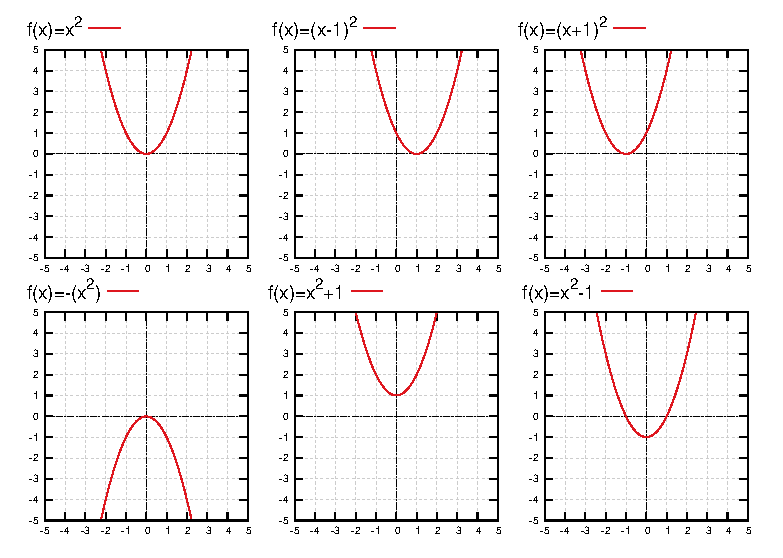
\includegraphics[width=1\textwidth]{images/graph_transformation.eps}\caption{\label{fig:graph_translation}{Translation und Spiegelung des Funktionsgraphen von $f(x)=x^2$}}
\end{figure}
\begin{comment}
# Graph Transformation (gnuplot)
set terminal postscript eps enhanced color font 'Helvetica,10'
set output 'graph_transformation.eps'
set multiplot layout 2,3
set yrange [-5:5]
set xrange [-5:5]
set zeroaxis linetype 5 linewidth 1.5 lc 'black'
set xtics 1
set ytics 1
set grid linecolor rgb '#cccccc' linetype 3 linewidth 0.5
set key left tmargin font 'Helvetica, 18'
set tics scale 1.25
f(x)= x**2
set style line 1 linecolor rgb '#dd181f' linetype 1 linewidth 2
plot f(x) title 'f(x)=x^2' with lines ls 1
plot f(x-1) title 'f(x)=(x-1)^2' with lines ls 1
plot f(x+1) title 'f(x)=(x+1)^2' with lines ls 1
plot -f(x) title 'f(x)=-(x^2)' with lines ls 1
plot f(x)+1 title 'f(x)=x^2+1' with lines ls 1
plot f(x)-1 title 'f(x)=x^2-1' with lines ls 1
\end{comment}

\subsection{Funktionsgraph}
Als Funktionsgraph einer Funktion $f$ bezeichnet man die Menge aller geordneten Paare $(x, f(x))$ aus den Elementen $x$ der Definitionsmenge und den zugehörigen Funktionswerten $f(x)$.

\subsection{Gerade und ungerade Funktionen}
Eine Funktion ist gerade wenn ihr Funktionsgraph symmetrisch zur y-Achse ist und ungerade, wenn ihr Funktionsgraph symmetrisch zum Ursprung ist.
\begin{itemize}
\item $f(x)$ gerade: $f(x)=f(-x)$ \quad z. B. $f(x)=x^2, \quad f(x)=|x|$
\item $f(x)$ ungerade: $f(-x)=-f(x)$  \quad z. B. $f(x)=x^3, \quad f(x)=x$
\end{itemize}

\subsection{Verkettung zweier Funktionen}
Zwei Funktionen $f \colon A \to B$ und $g \colon B \to C$, bei denen der Wertebereich der ersten Funktion mit dem Definitionsbereich der zweiten Funktion übereinstimmt, können verkettet werden. Die Verkettung oder Hintereinanderausführung dieser beiden Funktionen ist dann eine neue Funktion, die gegeben ist durch
\[ g \circ f \colon A \to C, \, x \mapsto (g \circ f)(x) = g(f(x)) \]
\subsubsection{Beispiele für die Verkettung von Funktionen}
a)\[f(x)=x^2, \quad g(x)=x-1,\quad g\circ f=g(f(x))=x^2-1 \]
b)\[f(x)=\frac{1}{x^2}, \quad g(x)=x^3+2,\quad g\circ f=g(f(x))={\left(\frac{1}{x^2}\right)}^3+2 \]
c)\[f(x)=\frac{x+1}{2x-3}, \quad g(x)=\frac{x-3}{x+1}, \quad g\circ f=g(f(x))=\frac{\frac{x+1}{2x-3}-3}{\frac{x+1}{2x-3}+1} \]

\subsection{Umkehrfunktion}
Die Umkehrfunktion erhält man durch Umformen und Auflösen der Funktionsgleichung nach x. Eine Umkehrfunktion existiert jedoch nur bei bestehender 1:1 Zuordnung zwischen Elementen der Definitionsmenge und  Zielmenge der Funktion. Die Zielmenge der Funktion ist die Definitionsmenge der Umkehrfunktion. \\\\
Sei $f: \mathbb{R} \to \mathbb{R}$ mit $f(x) = 2x - 1$. Die folgenden Gleichungen sind äquivalent:
\begin{align*} 
y = 2x - 1 \\
2x = y + 1 \\
x = \frac{y+1}{2} 
\end{align*}
Die Umkehrfunktion von f lautet daher $f^{-1}(y)=\frac{y+1}{2}$. Da es üblich ist, das Argument mit x zu bezeichnen, schreibt man auch: $f^{-1}(x)=\frac{x+1}{2}$. 

\subsection{Exponentialfunktion}
Die Exponentialfunktion ist eine Funktion der Form $x \mapsto a^x$ mit einer reellen Zahl $a > 0$ und $a \neq 1$ als Basis (Grundzahl). Im Gegensatz zu den Potenzfunktionen, bei denen die Basis die unabhängige Größe (Variable) ist, ist bei Exponentialfunktionen die Variable der Exponent (auch Hochzahl) des Potenzausdrucks. 
\[f(x)=c a^x \quad (a \in \mathbb{R}^+,c \in \mathbb{R}) \] heisst Exponentialfunktion zur Basis a.
\begin{figure}[h!]
\centering
\includegraphics[width=0.7\textwidth]{images/exponentialfunktion}\caption{\label{fig:exponentialfunktion}{Graph der Exponentialfunktion $y=e^x$ (rot) mit der Tangente (hellblau gestrichelte Linie) durch den Punkt 0/1}}
\end{figure}
\begin{itemize}
\item $f(x)=a^x$ ist streng monoton steigend wenn $a>1$
\item $f(x)=a^x$ ist streng monoton fallend wenn $a<1$
\end{itemize}

\subsection{Logarithmusfunktion}
Der Logarithmus zur Basis b ist die Umkehrfunktion der allgemeinen Exponentialfunktion zur positiven Basis b. Die Funktionen $b^x$ und $\log_b x$ sind also Umkehrfunktionen voneinander, d. h. Logarithmieren macht Exponenzieren rückgängig und umgekehrt:
\[ b^{\log_b x} = x \quad \text{und} \quad \log_b(b^x) = x \]
Der natürliche Logarithmus ergibt sich mit der Basis b=e, wobei
\[e = 2{,}718281828459\ldots\]
die eulersche Zahl ist.
\begin{figure}[h!]
\centering
\includegraphics[width=0.7\textwidth]{images/logarithmusfunktion}\caption{\label{fig:logarithmusfunktion}{Graph der Logarithmusfunktion zur Basis 2 (grün), e (rot) und 1/2 (blau)}}
\end{figure}

\section{Exponentielles Wachstum und Abklingen}
Exponentielles Wachstum beschreibt ein mathematisches Modell für einen Wachstumsprozess, bei dem sich die Bestandsgröße in jeweils gleichen Zeitschritten immer um denselben Faktor verändert. Der Wert der Bestandsgröße kann im zeitlichen Verlauf entweder steigen (exponentielle Zunahme) oder abnehmen (exponentieller Zerfall).
\[ N(t)=N_0a^t \quad \text{ oder } \quad N(t)=N_0e^{kt}\]
$k,a > 0$: steigend, $k,a < 0$: fallend, $N_0$: Anfangswert, \\ a: Wachstum pro Zeit, t: Zeit
\begin{itemize}
\item $a>1$: $a^h=1+\frac{P}{100}$
\item $a<1$: $a^h=1-\frac{P}{100}$ (P: Wachstum/Zerfall in Prozent)
\end{itemize}

\subsection{Verdopplungszeit}
Die Zeit für eine Verdopplung des Anfangswerts ergibt sich zu
\[ t = \frac{\ln 2}{\ln a} \quad (a>1) \]

\subsection{Halbwertszeit}
Die Zeit für eine Halbierung des Anfangswerts ergibt sich zu
\[ t = \frac{\ln \frac{1}{2}}{\ln a}  \quad (a<1) \]

\subsection{Beispiel für exponentielles Wachstum}
Bakterienstamm in Nährlösung, 11\% Wachstum pro Stunde. Anfangswert 500.
\\\\
Anzahl an Bakterien nach 8 Stunden
\begin{align*}
N(t)&=N_0a^t \\
N(t)&=500 \cdot (1,11)^t \\
N(8)&=500 \cdot (1,11)^8 \approx 1150
\end{align*}
Verdopplung des Anfangswerts nach 6,64 Stunden
\begin{align*}
t= \frac{\ln 2}{\ln {1,11} } \approx 6,64
\end{align*}

\section{Einheitskreis}
Der Einheitskreis ist ein Kreis dessen Radius die Länge 1 hat und dessen Mittelpunkt mit dem Koordinatenursprung eines kartesischen Koordinatensystems der Ebene übereinstimmt. Der Einheitskreis besteht also aus den Punkten $(x,y)$ der Ebene, für die $x^2 + y^2 = 1$ gilt.
\subsection{Punkte auf dem Einheitskreis}
Liegt ein Punkt P auf dem Einheitskreis, dann kann man einen Winkel $\varphi$ zu der x-Achse definieren, unter dem P vom Ursprung des Koordinatensystems aus gesehen wird. Für die Koordinaten $x_p$, $y_p$ von P gilt dann
\[ x_p = \cos \varphi, y_p = \sin \varphi \text{ und } y_p/x_p = \tan \varphi \]
\begin{align*}
\cos \varphi &= \frac{\text{Ankathete}}{\text{Hypotenuse}} = x \\
\sin \varphi &= \frac{\text{Gegenkathete}}{\text{Hypotenuse}} = y \\
\tan \varphi &= \frac{\text{Gegenkathete}}{\text{Ankathete}} = \frac{y}{x} \\
\cot \varphi &= \frac{\text{Ankathete}}{\text{Gegenkathete}} = \frac{x}{y}
\end{align*}

\subsection{Umrechnung zwischen Radiant und Grad}
Der Vollwinkel hat $2 \pi$ Radiant oder 360 Grad ($ 2\pi\,\mathrm{rad} = 360^\circ $), daher gilt
\[1^\circ = \frac{\pi}{180^\circ} \,\mathrm{rad} \]
\[1\,\mathrm{rad} = \frac{180^\circ}{\pi}\]

\begin{figure}[h!]
\centering
\includegraphics[width=1.1\textwidth]{images/einheitskreis}\caption{\label{fig:einheitskreis}{Punkte auf dem Einheitskreis}}
\end{figure}

\section{Folgen}
Als Folge wird in der Mathematik eine Auflistung von endlich oder unendlich vielen fortlaufend nummerierten Objekten bezeichnet. Dasselbe Objekt kann in einer Folge auch mehrfach auftreten. \\\\
Da unendliche Folgen nicht vollständig aufgelistet werden können, muss ein Bildungsgesetz für die Folgenglieder bekannt sein oder sich aus den aufgeschriebenen Anfangsgliedern zweifelsfrei ergeben. Unendliche Folgen können gegen einen Grenzwert konvergieren.

\subsubsection{Beispiele}
\begin{itemize}
\item $(1, 0, 0, 1, 1)$ 5-Tupel von ganzen Zahlen
\item $(\sin,\ \cos,\ \tan,\ \cot)$ 4-Tupel trigonometrischer Funktionen
\item $(2, 3, 5, 7, 11, 13, \dotsc)$ Folge der Primzahlen
\item $(\{\}, \{1\}, \{1,2\}, \{1,2,3\}, \dotsc)$ Unendliche Folge von Mengen
\item $(x_0, x_1, x_2, x_3, \dotsc)$ Allgemeine unendliche Folge, deren Terme fortlaufend indiziert sind.
\end{itemize}

\subsubsection{Funktionsvorschriften}
Die Folge der natürlichen Zahlen 0, 1, 2, 3, … Dieses Beispiel ist speziell, weil die Werte von Folgenglied und Index übereinstimmen. Die Funktionsvorschrift lautet einfach
\[ a_i = i \]
Die Folge der ungeraden Zahlen 1, 3, 5, 7, … hat die Funktionsvorschrift
\[ a_i = 2i+1\]
Die Folge der Zweierpotenzen 1, 2, 4, 8, …
\[ a_i = 2^i \]

\subsection{Beschränktheit}
Eine Folge heißt nach oben beschränkt, wenn sie eine obere Schranke S besitzt, so dass für alle i aus $\mathbb{N}$ gilt: $a_i \leq S$.  Die Begriffe nach unten beschränkt und untere Schranke sind analog definiert. Eine Folge die nach oben und unten beschränkt ist, heißt beschränkte Folge.

\subsection{Arithmetische Folgen}
Eine arithmetische Folge ist eine Folge mit konstanter Differenz zwischen aufeinanderfolgenden Gliedern. Der Graph einer arithmetischen Folge ist eine Gerade.
\begin{itemize}
\item Termdarstellung: $a_n=kn + d$
\item Rekursive Darstellung: $a_{n+1}-a_n = k$
\end{itemize}

\subsection{Geometrische Folgen}
In einer geometrischen Folge stehen aufeinanderfolgende Glieder in einem konstanten Verhältnis zueinander und es gilt
\[ b_n=b_0 \cdot q^n \]

\subsection{Grenzwerte von Folgen}
Nähern sich die Glieder einer Folge einer bestimmten Zahl a dann nennt man a den Grenzwert (Limes) der Folge und schreibt
\[ \lim_{n \to \infty} a_n=a \]
Für eine Folge  $a_n$ mit Grenzwert $\lim_{n \to \infty} a_n=a$ gilt
\[ \lim_{n \to \infty} (ca_n)=ca \]
\[ \lim_{n \to \infty} (c+a_n)=c+a \]
Folgen für die ein Grenzwert existiert nennt man konvergent, Folgen für die kein Grenzwert existiert heissen divergent.

\subsubsection{Beispiele für Grenzwerte von Folgen}
a) \[ \text{Folge } a_n=\frac{1}{n^2}: \quad \left(1,\frac{1}{4}, \frac{1}{9}, \frac{1}{16}, \cdots \right) \quad \text{Grenzwert: } \lim_{n \to \infty} \frac{1}{n^2}=0 \]
b) \[ \text{Folge } a_n=1-\frac{1}{n}: \quad \left(0, \frac{1}{2}, \frac{2}{3}, \frac{3}{4}, \cdots \right) \quad \text{Grenzwert: } \lim_{n \to \infty} 1- \frac{1}{n}=1 \]

\section{Reihen}
Eine Reihe ist als eine Folge definiert, deren Glieder die Partialsummen einer anderen Folge sind. Die n-te Partialsumme ist die Summe der ersten n  Summanden. \\\\
Falls die Folge dieser Partialsummen einen Grenzwert besitzt, so wird dieser der Wert oder die Summe der Reihe genannt.
Ist eine beliebige Folge $(a_i)$ gegeben, kann man aus ihr eine neue Folge $\left(s_n\right)$ konstruieren:
\[ s_n := a_0 + a_1 + \ldots + a_n \]
Diese Glieder der Folge heißen (n-te) Partialsummen. Die Folge $\left(s_n\right)$ dieser Glieder, also die Folge der n-ten Partialsummen heißt Reihe. Falls die Reihe konvergiert, so nennt man ihren Grenzwert Wert oder Summe der Reihe:
\[ \lim_{n \to \infty} s_n = \lim_{n \to \infty} \sum_{i=0}^n a_i \] 
Für eine endliche arithmetische Folge $(a_1+a_2+a_3+\cdots+a_n)$ gilt
\[ S=\frac{n}{2}(a_1+a_n) \]
Ist $b_1+b_2+\cdots+b_n$ eine endliche geometrische Reihe mit n Gliedern und Quotient $q \neq 1$ dann ist die Summe
\[ S=b_1 \frac{q^n-1}{q-1} \]

\section{Vektoren in $\mathbb{R}^3$}
\subsection{Addition und Subtraktion}
Für die Addition von Vektoren gilt das Kommutativ- und Assoziativgesetz.
\[
\vec a \pm \vec b=\begin{pmatrix}a_1\\a_2 \\a_3 \end{pmatrix} \pm \begin{pmatrix}b_1\\b_2 \\b_3 \end{pmatrix}=\begin{pmatrix}a_1 \pm b_1\\a_2 \pm b_2 \\ a_3 \pm b_3 \end{pmatrix} 
\]
\subsection{Multiplikation mit einem Skalar}
Vektoren können mit reellen Zahlen (Skalare) multipliziert werden.
\[
r\vec a=r\begin{pmatrix}a_1\\a_2\\a_3 \end{pmatrix}=\begin{pmatrix}ra_1\\ra_2\\ra_3 \end{pmatrix}
\]
\subsection{Multiplikation von Vektoren}
Das Produkt zweier Vektoren wird Skalarprodukt genannt. Das Ergebnis ist ein Skalar.
\[
\vec a \cdot \vec b=\begin{pmatrix}a_1\\a_2\\a_3 \end{pmatrix} \cdot \begin{pmatrix}b_1\\b_2\\b_3 \end{pmatrix}=a_1b_1+a_2b_2+a_3b_3
\]
\subsection{Betrag eines Vektors}
Der Betrag bzw. die Länge eines Vektors kann durch den Satz des Pythagoras berechnet werden.
\[
|\vec a| = \sqrt{a_1^2 + a_2^2 + a_3^2}
\]
\subsection{Einheitsvektor}
Ein Einheitsvektor ist ein Vektor der Länge Eins. Der Einheitsvektor eines Vektors wird durch Division des Vektors durch seinen Betrag berechnet.
\[
a_0 = \frac{\vec a}{|\vec a|}
\]
\subsection{Kreuzprodukt}
Das Kreuzprodukt (Vektorprodukt) lässt wie folgt berechnen:
\[
 \vec{a}\times\vec{b} = \begin{pmatrix}a_1 \\ a_2 \\ a_3 \end{pmatrix}\times\begin{pmatrix}b_1 \\ b_2 \\ b_3 \end{pmatrix} = \begin{pmatrix}a_2b_3 - a_3b_2 \\ a_3b_1 - a_1b_3 \\ a_1b_2 - a_2b_1 \end{pmatrix}
\]
Der erhaltene Vektor ist im rechten Winkel zu den Vektoren $\vec a$ und $\vec b$:
\[ \vec a \times \vec b \perp \vec a \]
\[ \vec a \times \vec b \perp \vec b \]
\subsection{Orthogonalität}
Zwei Vektoren $\vec a$ und $\vec b$ heissen orthogonal (zueinander im rechten Winkel), wenn ihr Skalarprodukt Null ist.
\[
\vec a \perp \vec b \Leftrightarrow \vec a \cdot \vec b = 0
\]
\subsection{Parallelität}
Zwei von 0 verschiedene Vektoren $\vec a$ und $\vec b$ sind zueinander parallel wenn sie Vielfache voneinander sind, es also einen Skalar $r \neq 0$ gibt, so dass $\vec b = r\vec a$.
\[
\vec a \parallel \vec b \Leftrightarrow \vec b = r \vec a
\]

\section{Geraden in $\mathbb{R}^3$}
Für Geraden in $\mathbb{R}^3$ gibt es keine Normalvektordarstellung. Die Parameterdarstellung einer Geraden im Raum hat die Form $g: X=P+t\cdot \vec g$
\[\begin{pmatrix} x_1 \\ x_2 \\ x_3\end{pmatrix}=\begin{pmatrix} p_1 \\ p_2\\ p_3 \end{pmatrix} + t\begin{pmatrix} g_1 \\ g_2\\ g_3\end{pmatrix}\]

\section{Ebenen in $\mathbb{R}^3$}
Eine Ebene ist definiert durch einen Punkt und zwei Richtungen.
Die Parameterdarstellung einer Ebene im Raum hat die Form $X=P+t\cdot \vec g + s \cdot \vec h$
\[\begin{pmatrix} x_1 \\ x_2\\ x_3 \end{pmatrix}=\begin{pmatrix} p_1 \\ p_2\\ p_3 \end{pmatrix} + t\begin{pmatrix} g_1 \\ g_2\\ g_3\end{pmatrix} + s\begin{pmatrix} h_1 \\ h_2\\ h_3\end{pmatrix} \]
Ein Vektor $\vec n$ heisst Normalvektor der Ebene E wenn $\vec n$ zu allen Richtungsvektoren von E normal ist. Die Normalvektordarstellung einer Ebene lautet
\[ \vec n \cdot X = \vec n \cdot P \]
Der Normalvektor $\vec n$ ergibt sich aus der Parameterdarstellung zu
\[ \vec n = \vec g \times \vec h \]

\section{Statistik}
Statistik ist die Lehre von Methoden zum Umgang mit quantitativen Informationen (Daten). Sie ist eine Möglichkeit, eine systematische Verbindung zwischen Erfahrung (Empirie) und Theorie herzustellen. Unter Statistik versteht man die Zusammenfassung bestimmter Methoden, um empirische Daten zu analysieren.
\subsection{Median}
Der Median oder Zentralwert ist ein Mittelwert für Verteilungen in der Statistik. Der Median einer Auflistung von Zahlenwerten ist der Wert, welcher an der mittleren Stelle steht, wenn man die Werte der Größe nach sortiert. \\\\ Zum Beispiel für die Werte 4, 1, 37, 2, 1 ist die Zahl 2 der Median, nämlich die mittlere Zahl in 1, 1, \underline{2}, 4, 37.
\subsubsection{Bestimmung des Medians}
Der Median teilt eine Liste von Werten in zwei Hälften. Er kann auf folgende Weise bestimmt werden:
\begin{itemize}
\item Alle Werte werden aufsteigend geordnet.
\item Wenn die Anzahl der Werte ungerade ist, ist die mittlere Zahl der Median.
\item Wenn die Anzahl der Werte gerade ist, wird der Median meist als arithmetisches Mittel der beiden mittleren Zahlen definiert, die dann Unter- und Obermedian heißen.
\end{itemize}
\subsubsection{Definition}
Vorraussetzung: Werte sind bereits der Größe nach aufsteigend sortiert.
\[ \tilde x =\begin{cases} x_\frac{n+1}{2} & n\text{ ungerade}\\ \frac {1}{2}\left(x_{\frac{n}{2}} + x_{\frac{n}{2} + 1}\right) & n \text{ gerade} \end{cases} \]

\subsection{Arithmetisches Mittel}
Das arithmetische Mittel (Durchschnitt) ist ein Mittelwert, der als Quotient aus der Summe aller beobachteten Werte und der Anzahl der Werte definiert ist. \\\\
Das arithmetische Mittel einer Menge von n Werten $x_1, x_2, \ldots , x_n$ ist definiert als
\[ \bar{x}_{\mathrm{arithm}} = \frac{1}{n} \sum_{i=1}^n{x_i} = \frac{x_1 + x_2 + \cdots + x_n}{n} \]
Das arithmetische Mittel aus 50 und 100 ist  $\tfrac{50+100}{2} = 75$.

\subsection{Geometrisches Mittel}
Das geometrische Mittel ist ein Mittelwert und ist ein Mittelmaß für Größen, von denen das Produkt anstelle der Summe interpretierbar ist, z. B. von Verhältnissen oder Wachstumsraten. Das geometrische Mittel der n Zahlen $x_1,x_2,\dotsc,x_n$ ist gegeben durch die n-te Wurzel des Produkts der n Zahlen:
\[ G(x_1,x_2,\dotsc,x_n)= \bar{x}_\mathrm{geom} = \sqrt[n]{\prod_{i=1}^n{x_i}} = \sqrt[n]{x_1 \cdot x_2 \dotsm x_n} 
\]
Das geometrische Mittel zweier Werte a, b ist $\sqrt{ab}$, z.B. von a=3 und b=300: $\sqrt{3 \cdot 300} = 30$
\end{document}